

In this section, we present our proposed approach to learning inverse dynamics with contacts.
We first formalize the problem as learning a mixture-of-experts model.
Then we detail how to implement Gaussian processes as the corresponding experts.

%=============================================================


\subsection{Learning a Mixture-of-Contacts}



	When learning the inverse dynamics with contacts (\eq\eqref{eq:tau_contact}), we assume that the (contact-free) inverse dynamics from \eq\eqref{eq:tau_nocontact} can be computed precisely, either from an analytical model or from a learned model~\cite{Nguyen-Tuong2011}.
    %
    In our experiments, we employ a learned GP model for this purpose.
    The reason for this choice are the unmodeled dynamics $\epsilon\,(\q,\dq,\ddq)$, which introduce substantial errors even in absence of contacts.
	%
	As a result of this contact-free inverse dynamics, only the model of the additional term of the external forces $\color{darkgreen}{\sum_{i \in\mathcal{C}} {\jacobian_i(\q)}\T \extForces_i}$ has to be learned.
    In this paper, we consider a robot that is provided with skin measurements~$\skinInput$ from the tactile sensors, force measurements~$\ftsForces$ from the force torque sensors (FTS) and the applied torques~$\torques$.
    A visual representation of these relevant components is shown in \fig\ref{fig:concept}.
	Predicting the external forces $\color{darkgreen}{\sum_{i \in\mathcal{C}} {\jacobian_i(\q)}\T \extForces_i}$ can be formalized as the regression task
  	%
	\begin{align}
		\outputMatrix = \regressionNo(\inputMatrix) + \epsilon\,,
		\label{eq:generic_regression_noise}
	\end{align}
	%    
	where $\outputMatrix = \textcolor{darkgreen}{\sum_{i \in\mathcal{C}} {\jacobian_i(\q)}\T \extForces_i}$ and  $\inputMatrix = [\q, \skinInput,\ftsForces]$ are the inputs. 
	Additionally, $\epsilon$ is an i.i.d. Gaussian measurement noise with mean~$0$ and variance~$\sigma_n$.
	Therefore, our regression problem is phrased as
  	%
	\begin{align}
		\outputMatrix =\textcolor{darkgreen}{\sum_{i \in\mathcal{C}} {\jacobian_i(\q)}\T \extForces_i}  = \regressionNo([\q, \skinInput,\ftsForces]) + \epsilon\,.
		\label{eq:regression}
	\end{align}
	%    
	%
	It is necessary to consider the skin as an input~$\skinInput$ since contacts with different parts of the body lead to different effects in the dynamics.
	Intuitively, $\skinInput$ is required to identify the position of the contact.
	The force/torque measurements~$\ftsForces$ could be avoided if we were interested in learning contacts that do not change between training and test time, which would restrict us to dealing with static objects, such as a rigid floor, walls or stationary obstacles.
	However, as this assumption is limiting, we include the force/torque measurements~$\ftsForces$ in our model.

	The resulting regression of \eq\eqref{eq:regression} is a highly complex task, due to the extremely high-dimensional space of the input $\inputMatrix \in \inputSpace$ (the skin measurements~$\skinInput$ alone account for hundreds of dimensions) and nonlinearity.
    We tackle this problem by rephrasing it as a problem of learning a mixture-of-experts model (``mixture of contacts'' in our case).
	With this model, we decompose \eq\eqref{eq:regression} as
	%
	\begin{align}
		\textcolor{darkgreen}{\sum_{i \in\mathcal{C}} {\jacobian_i(\q)}\T \extForces_i}  = \sum_{j\in\mathcal{J}} f_j([\q, \ftsForces]) + \epsilon\,,
		\label{eq:expertofmixtureregression}
	\end{align}
	%    
	where $\mathcal{J}$ is the set of active experts~$f_j$.
    %, which depends from $[\q, \skinInput]$.
	Note that the skin input~$\skinInput$ is no longer explicitly part of the inputs of the experts. 
    Hence, each single expert~$f_j$ is now sufficiently low-dimensional to be modeled independently, but at the same time the possibility of summing the contribution of each contact allows to account for complex behaviors.
    As single expert~$f_j$ we propose to use Gaussian processes mapping $[\q, \ftsForces] \mapsto {\jacobian_j(\q)}\T \extForces_j$.
    Detailed information regarding the GP models and their training are given in the next subsection.
    The purpose of the gating network is then to select the experts that are currently active and to add their contributions.    
    An illustration of our approach is shown in \fig\ref{fig:model}.
	For mixture-of-experts models it is required to design a suitable gating network that activates the relevant experts.
    In our case, this gating network can be considered a classifier $\mathcal{J} = g(\q, \skinInput,\ftsForces)$ that selects which contact is currently ongoing.
	For simple tasks, this gating network can be designed using heuristics (e.g., using thresholds on the activation of the tactile sensors). 
    Alternatively, for more complex systems an approach based on machine learning is more suitable. 
    %In the experimental section we also evaluate the learning of such gating network.
	%This automatic design is increasingly helpful for high number of skin sensor ($>1000$), where the manual design became increasingly complex.

%\todo[inline]{How do you define the experts? And how many do you need? Not mentioned.}

%\todo[inline,color=yellow]{Make sure the section headings are consistently capitalized.}

	%
	\begin{figure}[t]
		\centering
		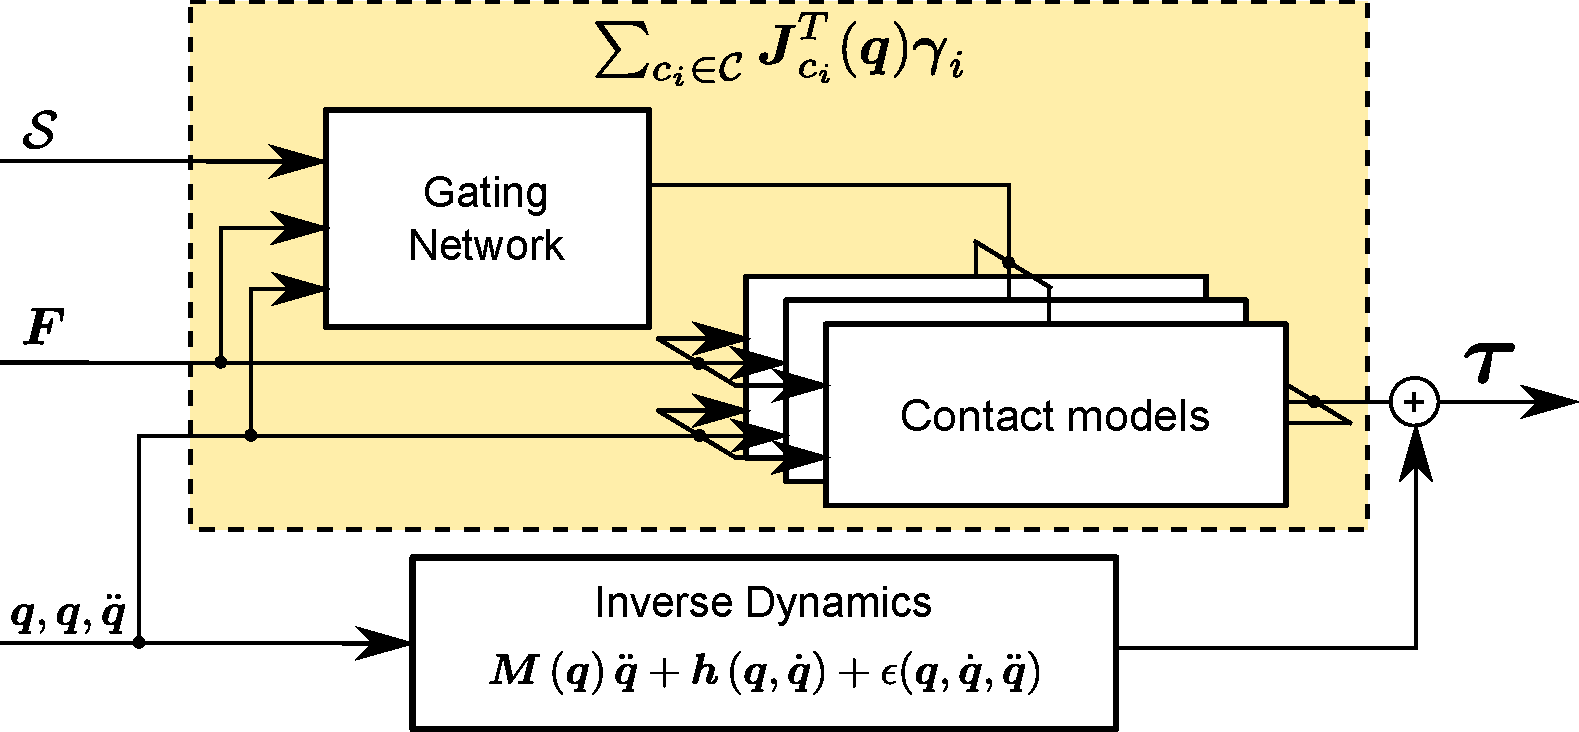
\includegraphics[width =.58\linewidth]{robertoIROS/fig/diagram_2.pdf}
		\caption{Our approach extends existing inverse dynamics without contacts by learning many contact models which serve as correction terms under different contacts type. The decision of which contact model to activate is taken by a gating network based on the skin measurements~$\skinInput$, the force torque sensors~$\ftsForces$ and the current state $\q, \dq, \ddq$.}
		\label{fig:model}
	\end{figure}
	%

%=============================================================


\subsection{Gaussian Processes as Expert Models}
%\todo[inline]{Introduce GPs only in the context of IDM: distribution over IDMs (instead of "function"), RBD as prior mean, define X and Y in this context immediately.}
	Gaussian Processes~\cite{Rasmussen2006} are a state-of-the-art regression method.
	They have been used in robotics to learn dynamics models~\cite{Deisenroth2012} and for control~\cite{Deisenroth2014}.
    %
    In the context of this paper, a GP is a distribution over inverse dynamics models 
	%
	\begin{align}
		f \sim \GP \left( m_f,k_f \right) \,,
	\end{align}
	%
	fully defined by a prior mean~$m_f$ and a covariance function~$k_f$.
	In our experiments, we choose as prior mean $m_f \equiv \torques_\text{RBD}$ and as covariance function~$k_f$ the squared exponential with automatic relevance determination and Gaussian noise:
    %
	\begin{align}
		{k(\vec x_p,\vec x_q)} &= \sigma_f^2\exp\left(\!-\!\tfrac{1}{2}(\vec x_p\! -\!\vec x_q)^T {\mat \Lambda\inv} (\vec x_p \!-\! \vec x_q)\right) \!+\! \sigma_w^2\delta_{pq}
		\label{sec:GP:cov:SE}
	\end{align}
	%
	where ${\mat \Lambda}=\diag([l^2_1,...,l^2_D])$ and $\delta_{pq}$ is the Kronecker delta (which is one if $p=q$ and zero otherwise). Here, $l_i$ are the characteristic length-scales, $\sigma^2_f$ is the variance of the latent function $f(\cdot)$ and $\sigma^2_w$ the noise variance. 
 %   The purpose of $\sigma_w^2\delta_{pq}$ is to model (and identify) the presence of the Gaussian noise~$\epsilon$.
    In our experiments, when learning contact models, the input is defined as $\parameters = [\q,\ftsForces]$ and the output (observations) is $\vec y = \torques$ are the torques.
    Hence, given $n$ training inputs $\mat X=[\parameters_1,...,\parameters_n]$ and corresponding training targets $\mat y=[ y_1,..., y_n]$, we define the training data set $\dataset = \{\mat X,\mat y\}$. 
    % training
Training the GP corresponds to finding good hyperparameters $\parameters = [l_i, \sigma_f, \sigma_w]$, which is done by the standard procedure of maximizing the marginal likelihood~\cite{Rasmussen2006}.   
    
% predictive distribution    
    The GP yields the predictive distribution over torques for a new input $\vec x_* = [\vec q_*, \mat F_*]$
	%
	\begin{align}
		&\prob(\vec y|\dataset,\parameters_*) = \gauss{\mu(\parameters_*)}{\sigma^2(\parameters_*)}\,, 
		\label{eq:one-step prediction distr}
	\end{align}
	%
	where the mean~$\mu(\parameters_*)$ and the variance~$\sigma^2(\parameters_*)$ are 
	%
	\begin{align}
		&\mu(\parameters_*) = \vec k^T_*\vec K^{-1} \mat y\,,\quad \sigma^2(\parameters_*) = k_{**}-\vec k^T_*\mat K^{-1}\vec k_*\,.
		\label{eq:one-step prediction mean and covariance}
		%\label{eq:one-step prediction cov}
	\end{align}
	%
	%% all the stuff from the equations
	The entries of the matrix $\vec K$ are  $K_{ij}= k(\parameters_i,\parameters_j)$, and we define $k_{**}=k(\parameters,\parameters)$ and $\vec k_{*}=k(\vec X,\parameters)$. 

%=============================================================

\subsection{Controlling the Contacts}

In the case of no contacts $\mathcal{C}=\{0\}$ we can define the Task-space Nonlinear Feedforward Control:
%
\begin{align}
	\vec u = \torques_\text{RBD}\,,
\end{align}
%
where the~$\torques_\text{RBD}$ is computed from the rigid body inverse dynamics (or a learned model of it).
Often an additional PD feedback controller is added to compensate for noise and inaccuracies in the dynamics, such that
%
\begin{align}
	\vec u = \torques_\text{RBD} + \underbrace{K_P \left(\q^{\text{des}}-\q\right) + K_D \left(\dq^{\text{des}} - \dq\right)}_{\torques_\textit{PD}}\,.
\end{align}
%
Intuitively, the magnitude of the torques contribution from the PD controller~$\torques_\textit{PD}$ can be used to measure the goodness of our inverse dynamics model.
Accurate inverse dynamics model will only need small corrections by the feedback controller, while inaccurate models will rely more heavily on it.
In case of inaccurate models increasing the PD gains can still lead to acceptable tracking performance at the expense of safety.
However, with unforeseen obstacles, high gains can lead to both damages to the robot's hardware and the obstacle itself.

% %=============================================================

% \subsection{Inverse Dynamics with External Forces}

% 	In this Section we describe the basics of Inverse Dynamics and Inverse Dynamics in presence of external forces.
    
%     Without contacts with the environment, the dynamics of a robot with $m$ degrees of freedom can be generally described by 
% %
% \begin{align}
% 	\torques = \underbrace{\inertiaMatrix\ddq + \Hmatrix}_{\torques_\text{RBD}} + \epsilon\,(\q,\dq,\ddq) \,,
% 	\label{eq:tau_nocontact}
% \end{align}
% %
% where $\q$, $\dq$ and $\ddq$ are  the joint positions, velocities and accelerations, respectively, $\inertiaMatrix \in \R^{m \times m}$ is the inertia matrix, and $\Hmatrix \in \R^{m \times m}$ is the matrix combining the contributions from Coriolis and centripetal, friction (viscous and static) and gravity forces:
% %
% \begin{align}
% 	\Hmatrix = C(\q,\dq)\dq + g(\q) + F_v \dq + F_s \,\text{sgn}(\dq) \,.
% \end{align}
% %
% The term $\epsilon(\q,\dq,\ddq)$ in \eq\eqref{eq:tau_nocontact} captures the errors of the model, such as unmodeled dynamics (e.g., elasticities and Stribeck friction), inaccuracies in the dynamic parameters (e.g., masses, inertia), vibrations, couplings, and sensor noise. 

% With a set $\mathcal{C}=\{c_1 \ldots c_n\}$ of contacts $c_i$ between the robot and the environment, \eq\eqref{eq:tau_nocontact} becomes
% %
% \begin{align}
% 	\torques = \underbrace{\inertiaMatrix\ddq + \Hmatrix}_{\torques_\text{RBD}} + \epsilon(\q,\dq,\ddq) + \color{darkgreen}{\sum_{c_i \in\mathcal{C}} {\jacobian\T_{c_i}(\q)}\, \extForces_i} \,\color{black}{,}
% 	\label{eq:tau_contact}
% \end{align}
% %
% where the last term accounts for the effect of the external wrenches (forces and moments) $\extForces_i$ applied at the contact location $c_i$, and $\jacobian_{c_i}(\q)$  is the contact Jacobian\footnote{The contact location $c_i$ is not necessarily fixed, as the contacts may occur on the whole robotic structure and not exclusively at the end-effectors. 
% In such a case, the contact location, if not known a priori, must be estimated, typically through distributed tactile sensors.
% To compute the contact Jacobian, we need the position of the contact point with respect to the reference frame of the link~\cite{Fumagalli2012}. 
% Such a knowledge requires a kinematic calibration of the skin, as explained in~\cite{DelPrete2011}.}.



% %=============================================================

% \subsection{Learning Inverse Dynamics with Tactile Sensing}

% 	In this Section we explain how we can learn the inverse dynamics in presence of contacts using GPs


% %=============================================================

% \subsection{Controlling the Contacts}

% In the case of no contacts $\mathcal{C}=\{0\}$ we can define the Task-space Nonlinear Feedforward Control:
% %
% \begin{align}
% 	\tau_{\text{M}} &= \color{red}{\tau_{\text{FF}}} \color{black}{+} \color{blue}{\tau_{\text{FB}}} \color{black}{\,,}\\
% 	\color{red}{\tau_{\text{FF}}} &= u_{\text{IDM}} (\q^{\text{des}},\dq^{\text{des}},\ddq^{\text{des}})\,,\\
% 	\color{blue}{\tau_{\text{FB}}} &= K_P(\q^{\text{des}}-\q) + K_D (\dq^{\text{des}} - \dq)\,.
% \end{align}

% %=============================================================
